\section{Backlog/roadmap du sprint Alpha}

L’objectif de ce sprint est de poser les fondations et délivrer les fonctionnalités de bases attendues par l’utilisateur,
c'est-à- dire la compréhension des dispositions possibles et impossibles.

Pour ce faire le backlog suivant a été "embarqué" dans cette version et a résulté en la roadmap suivante:

\begin{center}
      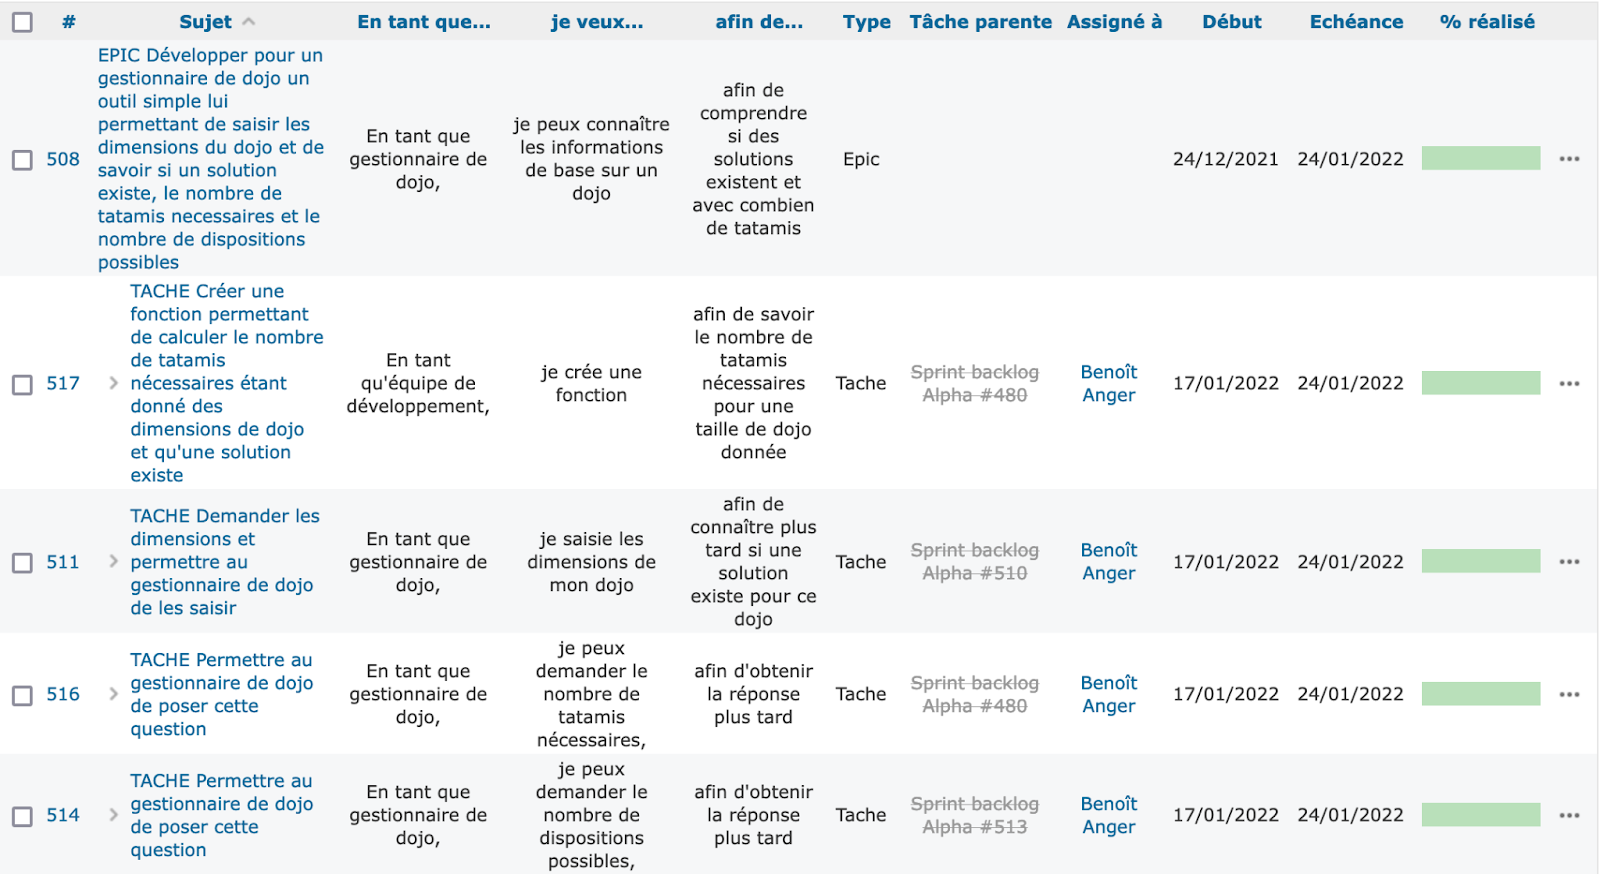
\includegraphics[width=17cm]{images/roadmap-alpha-part1.png}
\end{center}

\begin{center}
      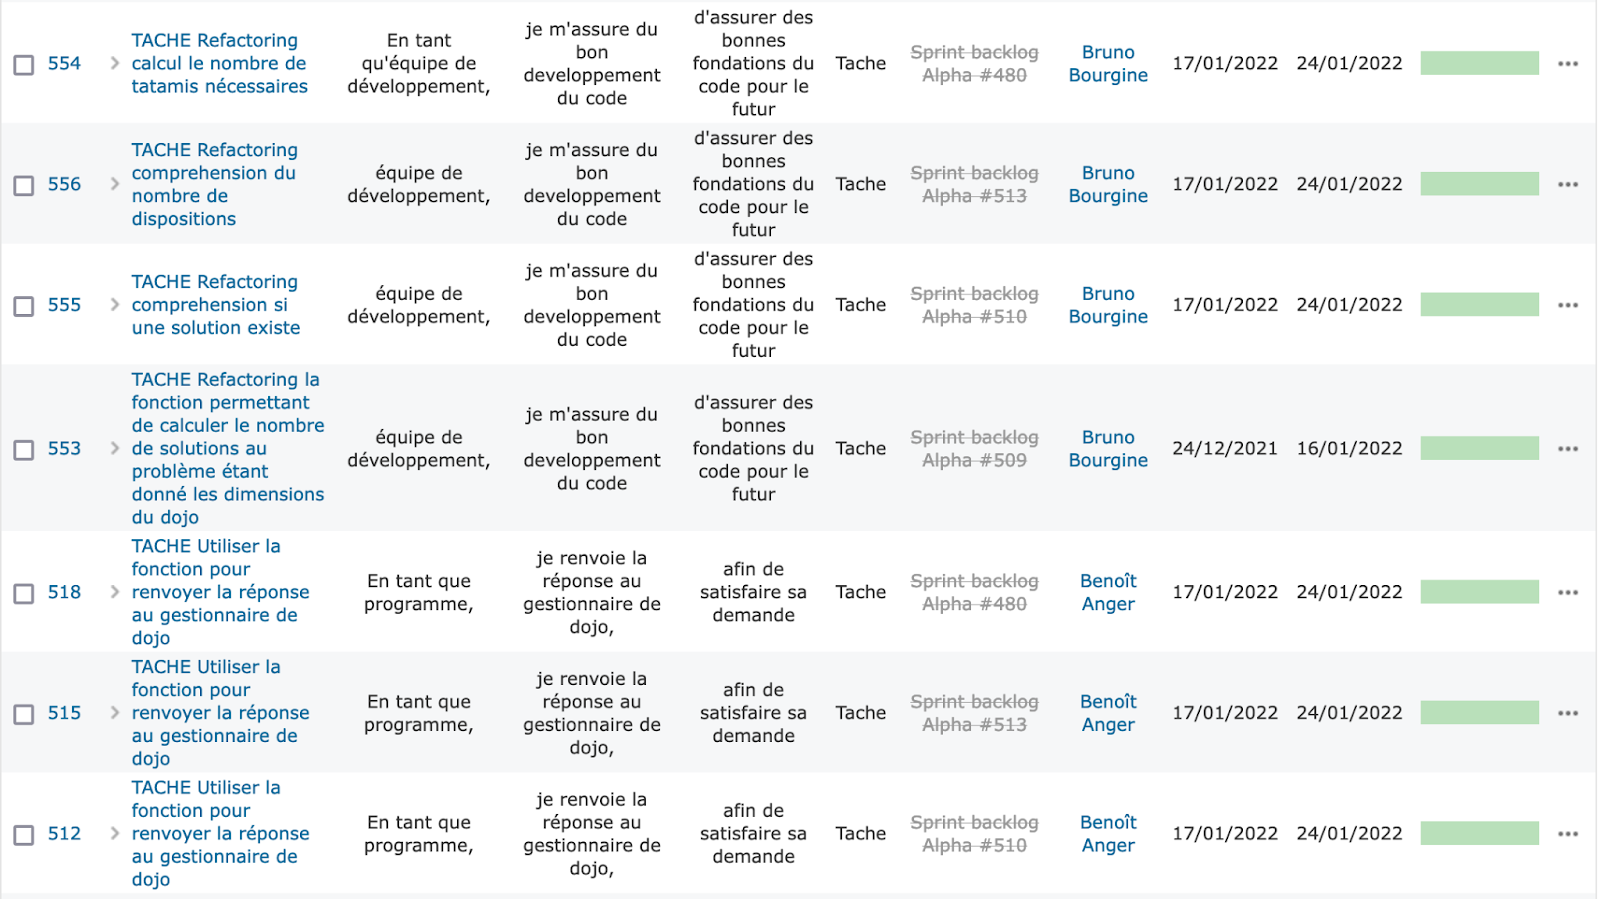
\includegraphics[width=17cm]{images/roadmap-alpha-part2.png}

      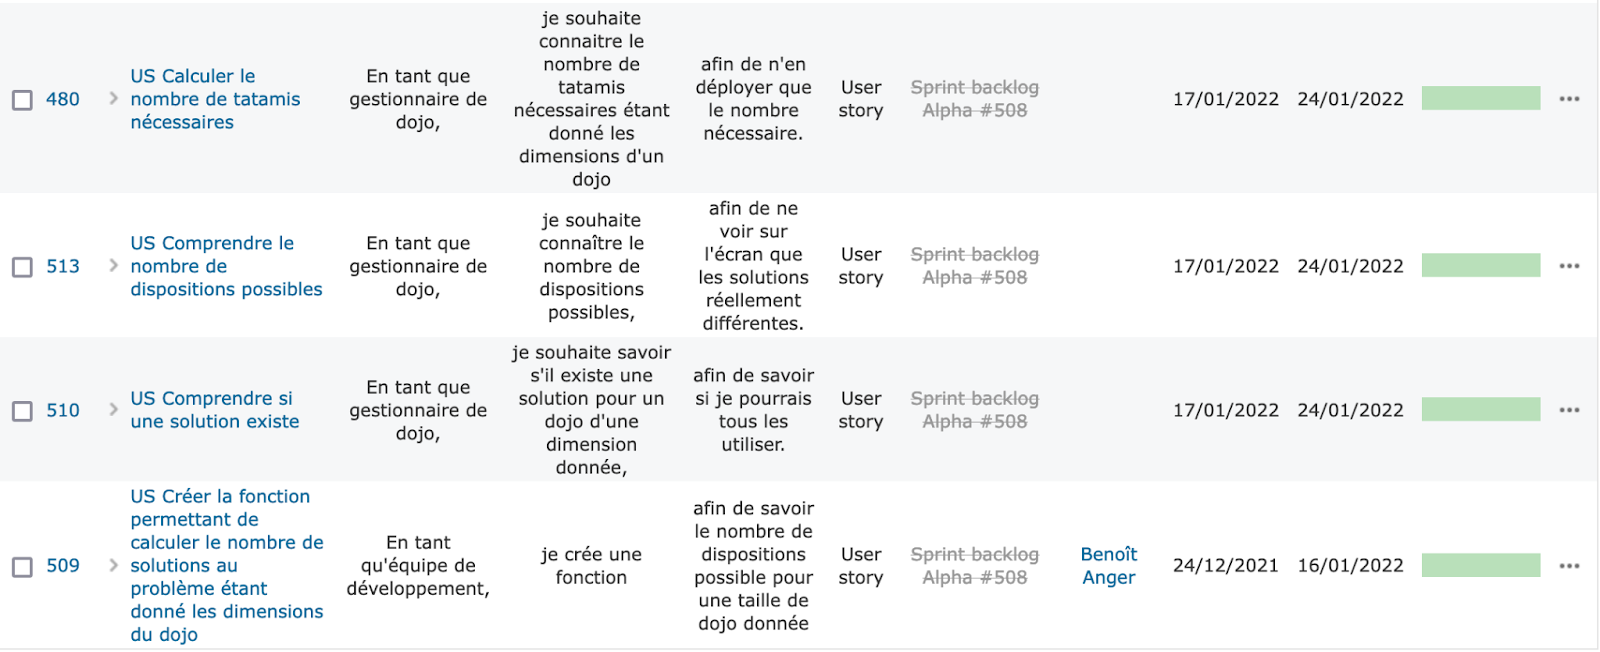
\includegraphics[width=17cm]{images/roadmap-alpha-part3.png}
\end{center}

\newpage
Et ici présenté en diagramme de Gantt:

\begin{center}
    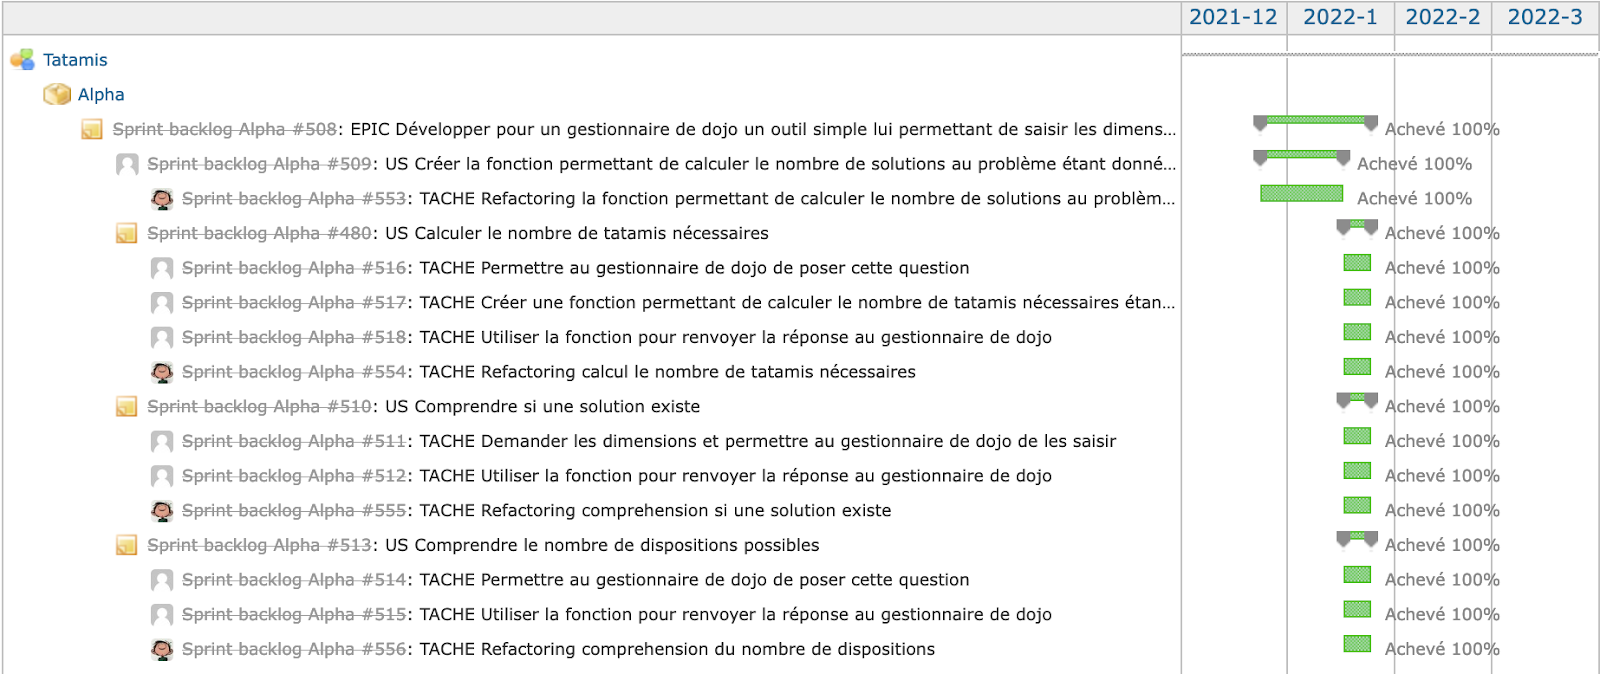
\includegraphics[width=16cm]{images/tatamis-gantt-alpha.png}
\end{center}

\section{Tests}


\noindent%
\begin{adjustwidth}{-1.5cm}{0cm}

    \renewcommand{\arraystretch}{1.2}
    {\setlength{\tabcolsep}{1.5 mm}
        \begin{testtabular}{|m{0.6cm}|m{5.5cm}|m{8cm}|m{2cm}|c|} \hline
            \rowcolor{tssteelblue} \textcolor{white}{id}                        & \textcolor{white}{Sujet}                                                                   & \textcolor{white}{Test d'acceptance (en gris : test utilisateur)}                                                                                            & \textcolor{white}{Méthode de test} & \textcolor{white}{Résultat} \\ \hline
            518                                                                            & TACHE Utiliser la fonction pour renvoyer la réponse au gestionnaire de dojo          &
            Quand le programme est lancé et que l'utilisateur saisi comme attendu,
            une réponse lui est renvoyée dans la console                                   & Manuel                                                                               & OK                                                                                                                                    \\ \hline
            517                                                                            & TACHE Créer une fonction permettant de calculer le nombre de tatamis nécessaires
            étant donné des dimensions de dojo et qu'une solution existe                   &
            Quand la fonction est exécutée, elle retourne le nombre de tatamis nécessaires &
            Automatisé                                                                     & OK                                                                                                                                                                                                                           \\ \hline
            \multirow{3}{0.6cm}{516}                                                       & \multirow{3}{5.5cm}{TACHE Permettre au gestionnaire de dojo de poser cette question} & 1. Quand le programme est lancé, il demande a l'utilisateur la largeur du dojo                           & Automatisé      & OK       \\ \cline{3-5}
            &                                                                                      & 2. Quand le programme est lancé, il demande a l'utilisateur la longueur du dojo                          & Automatisé      & OK       \\ \cline{3-5}
            &                                                                                      & 3. Quand le programme est lancé, une option est disponible pour l'utilisateur pour poser cette question. & Automatisé      & OK       \\ \hline
            515                      & TACHE Créer une fonction permettant de calculer le nombre de tatamis nécessaires étant donné des dimensions de dojo et qu'une solution existe & Quand la fonction est executée, elle retourne le nombre de tatamis nécessaires                                                                                                                                             & Automatisé      & OK       \\ \hline

            \multirow{3}{0.6cm}{514} & \multirow{3}{5.5cm}{TACHE Permettre au gestionnaire de dojo de poser cette question}                                                          & 1. Quand le programme est lancé, il demande à l'utilisateur la largeur du dojo                                                                                                                                             & Automatisé      & OK       \\ \cline{3-5}
            &                                                                                                                                               & 2. Quand le programme est lancé, il demande à l'utilisateur la longueur du dojo                                                                                                                                            & Automatisé      & OK       \\ \cline{3-5}
            &                                                                                                                                               & 3. Quand le programme est lancé, une option est disponible pour l'utilisateur pour poser cette question.                                                                                                                   & Automatisé      & OK       \\ \hline
            \multirow{2}{0.6cm}{513} & \multirow{2}{5.5cm}{US Comprendre le nombre de dispositions possibles}                                                                        & \cellcolor{tsgrey} 1. Étant donné que l'utilisateur saisie des dimensions de dojo, quand il saisie 2, il obtient le nombre conformément à l'article de Ruskey et Woodcock de 2009                                        & Automatisé      & OK       \\ \cline{3-5}
            &                                                                                                                                               & \cellcolor{tsgrey} 2. Étant donné que l'utilisateur saisie des dimensions de dojo en inversant la longueur et la largeur, quand il saisie 2, il obtient le nombre conformement a l'article de Ruskey et Woodcock de 2009 & Automatisé      & OK       \\ \hline


      
      
      \end{testtabular}}
\end{adjustwidth}



\noindent%
\begin{adjustwidth}{-1.5cm}{0cm}

    \renewcommand{\arraystretch}{1.2}
    {\setlength{\tabcolsep}{1.5 mm}
        \begin{testtabular}{|m{0.6cm}|m{5.5cm}|m{8cm}|m{2cm}|c|} \hline
            \rowcolor{tssteelblue} \textcolor{white}{id}                        & \textcolor{white}{Sujet}                                                                   & \textcolor{white}{Test d'acceptance (en gris : test utilisateur)}                                                                                            & \textcolor{white}{Méthode de test} & \textcolor{white}{Résultat} \\ \hline
            512                      & TACHE Utiliser la fonction pour renvoyer la réponse au gestionnaire de dojo	Alpha                                                              & Quand le programme est lancé et que l'utilisateur saisie comme attendu, une réponse lui est renvoyée dans la console                                                                                                       & Automatisé      & OK       \\ \hline
            \multirow{2}{0.6cm}{511} & \multirow{2}{5.5cm}{TACHE Demander les dimensions et permettre au gestionnaire de dojo de les saisir}                                         & 1. Quand le programme est lancée, il demande a l'utilisateur la largeur du dojo                                                                                                                                            & Automatisé      & OK       \\ \cline{3-5}
            &                                                                                                                                               & 2. Quand le programme est lancé, il demande a l'utilisateur la longueur du dojo                                                                                                                                            & Automatisé      & OK       \\ \hline
            \multirow{2}{0.6cm}{510} & \multirow{2}{5.5cm}{US Comprendre si une solution existe}                                                                                     & \cellcolor{tsgrey} 1. Etant donné que l'utilisateur saisie des dimensions de dojo n'ayant pas de solution, quand il saisie 1, il obtient 'Il n'existe pas de disposition possible avec des tatamis 2x1 pour ce dojo'     & Automatisé      & OK       \\ \cline{3-5}
            &                                                                                                                                               & \cellcolor{tsgrey} 2. Étant donné que l'utilisateur saisie des dimensions de dojo ayant au moins une disposition, quand il saisie 1, il obtient 'Il existe au moins une disposition avec des tatamis 2x1 pour ce dojo'   & Automatisé      & OK       \\ \hline

            \multirow{2}{0.6cm}{509}                                                                                 & \multirow{2}{5.5cm}{US Créer la fonction permettant de calculer le nombre de solutions au problème étant donné les dimensions du dojo} & 1. Quand la fonction est exécutée, elle retourne le nombre de dispositions possibles conformément a l'article de Ruskey et Woodcock de 2009                                        & Automatisé      & OK       \\ \cline{3-5}
            &                                                                                                                                        & 2. Quand la fonction est exécutée en inversant la longueur et la largeur, elle retourne le nombre de dispositions possibles conformément a l'article de Ruskey et Woodcock de 2009 & Automatisé      & OK       \\ \hline

            509                                                                                                      & EPIC Développer pour un gestionnaire de dojo un outil simple lui permettant de saisir les dimensions du dojo et
            de savoir si un solution existe, le nombre de tatamis nécessaires et le nombre de dispositions possibles & \cellcolor{tsgrey} cf. tests utilisateurs des US                                                                                     &                                                                                                                                                                                    &                            \\ \hline
            \multirow{2}{0.6cm}{480}                                                                                 & \multirow{2}{5.5cm}{US Calculer le nombre de tatamis nécessaires}                                                                      & 1. Étant donne que l'utilisateur saisit des dimensions de dojo avec une solution qui existe, quand il saisie 3, il obtient le nombre de tatamis nécessaires                        & Automatisé      & OK       \\ \cline{3-5}
            &                                                                                                                                        & 2. Étant donne que l'utilisateur saisit des dimensions de dojo avec aucune disposition possible, quand il saisie 3, il obtient un message indiquant l'absence de solution          & Automatisé      & OK       \\ \hline
        \end{testtabular}}
\end{adjustwidth}



\bigskip

Les tests automatisés sont définis dans le fichier \texttt{test\_alpha.py} et \texttt{test\_interface.py}. Ils peuvent être reproduits
en l'exécutant avec ligne de commande \texttt{python3 -m pytest}.


\section{Documentation utilisateur Alpha}

\subsection{Prérequis}

Configuration et installations requises:

\begin{itemize}
    \item Python 3.9 ou supérieur
    \item Librairies Python: aucune
\end{itemize}

\subsection{Comment trouver le nombre de tatamis nécessaires pour remplir un dojo?}

\begin{enumerate}
    \item Lancer le programme dans un Terminal (ligne de commande: \texttt{python3 interface.py})
    \item Entrer (dans le Terminal) la longueur et la largeur du dojo en suivant les questions posées par
          le programme. Nb: \textit{Vous pouvez inverser la longueur et la largeur, cela n’a pas d’importance}
    \item Répondre "3" à la question du programme “Que cherchez vous?”
    \item Interpréter la réponse:
          \begin{enumerate}
              \item \textbf{Réponse} : “Le nombre de tatamis 2x1 nécessaires pour ce dojo est : [Nombre]”.
                    \textbf{Interprétation}: il existe au moins une disposition possible et vous aurez besoin
                    d’exactement [Nombre] tatamis pour remplir le dojo.
              \item \textbf{Réponse} : “Il n'existe pas de disposition possible avec des tatamis 2x1 pour ce dojo”.
                    \textbf{Interprétation}: il n’existe aucune disposition possible de tatamis 2 x 1 pour remplir le dojo.
          \end{enumerate}
\end{enumerate}


\subsection{Comment savoir s’il existe une disposition possible de tatamis pour un dojo donné?}

\begin{enumerate}
    \item Lancer le programme dans un Terminal (ligne de commande: \texttt{python3 interface.py})
    \item Entrer (dans le Terminal) la longueur et la largeur du dojo en suivant les questions posées par
          le programme. Nb: \textit{Vous pouvez inverser la longueur et la largeur, cela n’a pas d’importance}
    \item Répondre "1" à la question du programme “Que cherchez vous?”
    \item Interpréter la réponse:
          \begin{enumerate}
              \item \textbf{Réponse} : “Il existe au moins une disposition avec des tatamis 2x1 pour ce dojo”.
                    \textbf{Interprétation}: il existe au moins une disposition possible.
              \item \textbf{Réponse} : “Il n'existe pas de disposition possible avec des tatamis 2x1 pour ce dojo”.
                    \textbf{Interprétation}: il n’existe aucune disposition possible de tatamis 2 x 1 pour remplir le dojo.
          \end{enumerate}
\end{enumerate}



\subsection{Comment savoir combien il existe de dispositions possibles de tatamis pour un dojo donné?}

\begin{enumerate}
    \item Lancer le programme dans un Terminal (ligne de commande: \texttt{python3 interface.py})
    \item Entrer (dans le Terminal) la longueur et la largeur du dojo en suivant les questions posées par
          le programme. Nb: \textit{Vous pouvez inverser la longueur et la largeur, cela n’a pas d’importance}
    \item Répondre "2" à la question du programme “Que cherchez vous?”
    \item Interpréter la réponse:
          \begin{enumerate}
              \item \textbf{Réponse} : “Il existe [Nombre] dispositions possibles”.
                    \textbf{Interprétation}: des dispositions existent pour ce dojo et il y en a [Nombre].
              \item \textbf{Réponse} : “Il existe 0 disposition possible”.
                    \textbf{Interprétation}: il n’existe pas de disposition pour ce dojo.
          \end{enumerate}
\end{enumerate}



\section{Explication des algorithmes et choix de programmation}

\subsection{Algorithme pour les calculs de nombre de dispositions}

Nous avons tenté deux approches pour répondre à ces fonctionnalités de base:

\begin{enumerate}
    \item Exploitation de la bibliothèque facile écrite en python pour résoudre des problèmes en programmation
          par contrainte. La publication de Xavier Olive\footnote{\url{https://www.xoolive.org/2016/02/29/pavage-par-tatamis.html}}
          proposant une application de cette  bibliothèque au problème qui nous concerne,nous avons explorer
          la possibilité d’adapter le programme proposé dans la publication. Si le nombre de dispositions proposées
          lors des calculs pour des dimensions de dojo données est tout à fait cohérent avec les valeurs trouvées
          dans les autres publications traitant de ce problème, il nous est rapidement apparu que les dimensions étaient limités,
          et que le temps de calcul n’était pas satisfaisant.
    \item Application de l’approche proposée par Dean Hickerson\footnote{Filling rectangular rooms with Tatami mats, 2002}:
          nous avons codé le programme mathématique qu’il décrit en python.

          La méthode 2 a finalement été retenue car elle a l’avantage d'être très légère et rapide en exécution.
          Elle peut notamment calculer rapidement des réponses même si les dimensions sont grandes (nous n’avons d’ailleurs par
          limites les dimensions saisies à un certain nombre).
\end{enumerate}



\subsection{Choix de programmation Interface}

Pour faire à l'essentiel, il a été choisi d'utiliser le terminal pour les interactions entre l'utilisateur et le programme.
Ce n’est évidemment pas idéal, mais cela a permis de rapidement traiter la partie interface pour se concentrer sur
les fonctionnalités et les calculs mathématiques permettant d’y répondre.

\subsection{Choix de la structure du programme}

Il nous semble important de suivre et mettre en application des principes \emph{SOLID}, et en particulier du
\emph{Single Responsibility Principle} et \emph{Open-Closed Principle}.
A ce stade, vu la simplicité du programme, ce n’est pas forcément nécessaire ni applicable de manière évidente,
mais nous souhaitons construire des fondations solides pour la suite:
\begin{itemize}
    \item Un fichier a une fonction principale

          Dans cette version alpha, nous avons 2 fichiers (un fichier de front-end \texttt{interface.py} et
          un fichier de back-end \texttt{alpha.py}) :
          \begin{itemize}
              \item \texttt{interface.py} : fichier contient toutes les fonctionnalités de front-end, c’est à dire
                    l’interface utilisateur
              \item \texttt{alpha.py} : fichier qui reprend les fonctions de calculs (basiques) de back-end
          \end{itemize}

\end{itemize}


\section{Challenges rencontrés et apprentissage}

\subsection{Challenges rencontrés et solutions appliquées}

Les deux challenges principaux de cette version ont été les suivants:

\begin{enumerate}
    \item Challenges techniques

          Bien que pas très exigeante techniquement, cette version pose les fonctionnalités de base sur lesquelles
          les versions suivantes reposent. En ce qui concerne les algorithmes, le challenge principal a été la recherche
          de la documentation qui prend du temps. Mais bien que cela ait demandé du temps, nous avons eu la chance de
          trouver beaucoup de documentation de bonne qualité sur le sujet des tatamis. Il nous a ensuite été relativement
          facile d'implémenter et tester les solutions trouvées. notamment car l'article de Dean Hickerson détaille les 
          formules mathématiques qui ont eu simplement à être transcrites en Python.

    \item Challenges organisationnels

          Bien que la coopération au sein de l'équipe ait débuté en phase de pré-développement, ce sprint était le premier
          qui impliquait un travail réel sur le code qui pose forcément de nouveaux challenges. Nous avons par ailleurs perdu
          définitivement un membre de l'équipe, impliquant inévitablement plus de travail de la part des membres restants.
          Pour nous permettre de bien avancer, nous avons mis en application les principes organisationnels suivants:
          \begin{itemize}
              \item Sessions de travail régulières (hebdomadaires) pour discuter des points ouverts et répartir
                    les tâches. Fréquence plutôt élevée pour garder un bon rythme de travail et éviter les à-coups.
              \item Retranscription écrite claire des tâches à effectuer avec les dates butoirs (et dépend-ances
                    de tâches lors qu’il y en a) avec un Compte Rendu écrit pour chaque session de travail
              \item Communication entre les sessions de travail (par Slack), notamment pour les discussions sur
                    l'exécution des tâches pré-requises à d'autres tâches dépendantes.
              \item Travail personnel entre les session pour accomplir les tâches

          \end{itemize}

          Par ailleurs, pour gérer le code, github (intégré à Slack pour recevoir les notifications lors des updates)
          a été utilisé.

\end{enumerate}


\subsection{Apprentissage}

Les enseignements principaux de ce sprint sont les suivants:

\begin{enumerate}
    \item Le choix de méthodologie agile confirmé comme étant la bonne approche pour travailler sur le projet.
    \item La perte d’un membre de l'équipe aurait notamment été plus difficile à gérer si tout avait été planifié 
    de manière rigide au départ
    \item Le bon fonctionnement de la coopération et organisation choisie (régularité des sessions de travail, documentation des sessions
    de travail avec des tâches et dates butoirs claires,...)
\end{enumerate}